\chapter{Results} \label{results}
This chapter will encompass the result of the two ML models for NBRA prediction in Instagram and Flickr media objects as well as the evaluation of the in-situ interviews and the passive observation statistic of NBRAs.
\section{Data-processing} \label{results_dataprocessing}
The following table \ref{tab:data_reduction_values}will provide data-reduction values for each data-source and dataset used. These reductions were the result of the different data-processing steps described in \ref{data_processing} which will be shortly listed again below:
\begin{itemize}
  \item in boundary check
  \item dominant authors exclusion
  \item bulk uploads
\end{itemize}

\begin{table}[h!]
\begin{center}
\caption{Data-reduction according to the different data-sources as a result of data-processing steps}\vspace{1ex}
\label{tab:data_reduction_values}
\begin{tabular}{ccccc}\hline
dataset & excluded top authors & bulk threshold & input & output & data-reduction\\ \hline
Instagram Zug & 6 & 6 & 28'246 & 11'777 & 58.3\% \\
Instagram Zurich Uetliberg & 10 & 5 & 74'742 & 68'522 & 8.3\% \\
Instagram Zurich Dolder & 7 & 5 &  206'454 &  191'584 & 7.2\% \\
Flickr Zug & 12 & 7 &  14'236 &  3'790 & 73.4\% \\ 
Foursquare Zug & - & - & 405 & 405 & 0.0\% \\ \hline
\end{tabular}
\end{center}
\end{table}

The noticeably high data-reduction of the Flickr dataset was mostly due to high user upload activity. As seen in figure \ref{img:dominant_users_flickr} a small portion of Flickr-users (authors) uploading up to  1'190 posts since the SMP Flickr was launched in 2005 account for a big share of the entire dataset. As a result to reduce this bias, roughly 5'700 media objects were removed alone in the 'dominant user' data-processing step.\\
Similar graphs to figure \ref{img:dominant_users_flickr} were created for all the datasets according to which the thesis author decided the thresholds in \ref{tab:data_reduction_values} manually. 

\begin{figure}[h!]
   \centering
   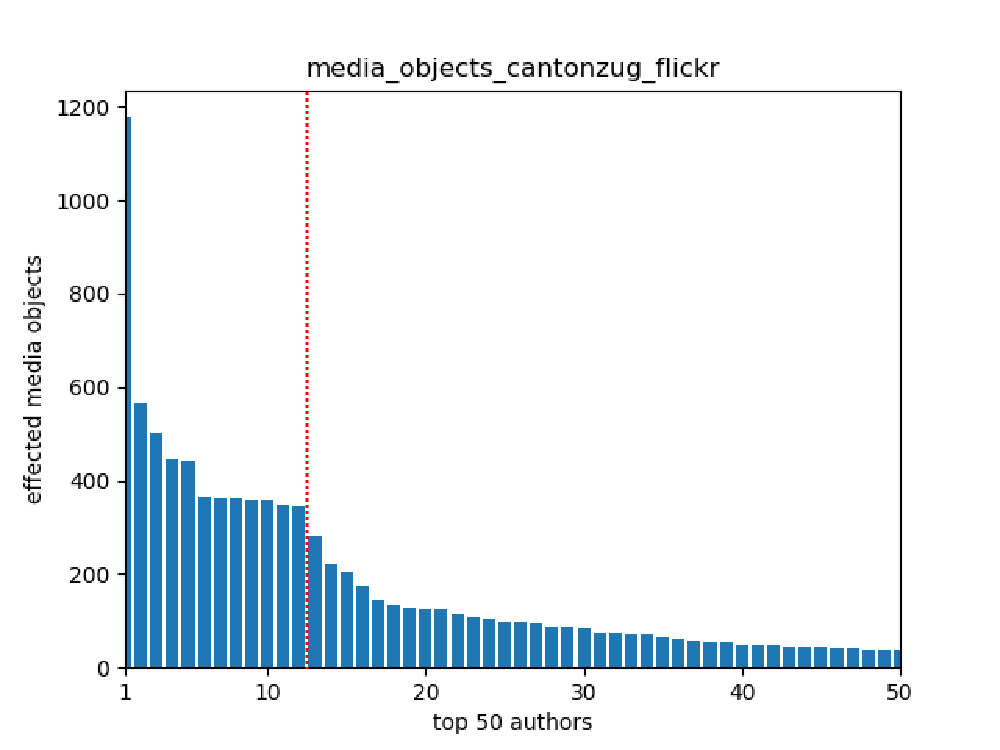
\includegraphics[width=0.75\textwidth]{img/cantonzug_flickr_top50_w_line}
   \caption{The top 12 Flickr authors which account for roughly 5'700 media objects (left to the red line) were excluded from further data-analysis}
   \label{img:dominant_users_flickr}
\end{figure}

\section{Models} \label{results_models}
The following subsections will cover the  performance results of each of the two created models (see chapter \ref{ml_model} that were solely trained on the Instagram Zurich Dolder and Instagram Zurich Uetliberg datasets included in the database table:\\ \texttt{media\_objects\_trainingdata\_instagram} (see figure \ref{database_setup}). For each model the random forest classifier and the linearSVC fitting algorithm was independently tested. The hyperparameters were tuned to yield the best possible average F1-score over all classes excluding the None-class. Simultaneously, the effect of including different amounts of the None-class training's data media objects during model fitting were also investigated. These values ranged from 500 to 6'500 with steps of 500.\\
These models were then used to predict the NBRAs contained in the media objects of the Instagram database table: \texttt{media\_objects\_unionzug\_instagram} and the \\Flickr database table: \texttt{media\_objects\_cantonzug\_flickr} from the Canton Zug.\\
Each model performed two separate predictions on each of the above mentioned datasets which differed in the final text-string composition that was parsed for prediction. One time the final text-string was constructed by concatenating the processed text-data and the image labels of a given media object. The second time the final text-string only contained the processed text-data.

\texttt{Remark:} The entire data presented in the following subchapters is available on the enclosed CD to this thesis. This includes the actual M1 and M2 dump files, tuning and cross-validation logs as well as the most important performance graphs (see chapter \ref{CD_content}).

\subsection{Model 1: untrained on image labels}
The first model (M1) that was trained exclusively on the processed user generated text-data (see chapter \ref{text_processing}). Therefore, it did not include any information about the image and its content. This leads to the model vocabulary potentially missing the associated image labels that the image recognition would yield.

\subsubsection{M1 - Random forest}
The model tuning with the parameter grid visible in figure \ref{code:randomForest_parameters} resulted in the following best hyper-parameter performing constellation:\\

\begin{table}[h!]
\begin{center}
\caption{Best hyperparameter setting for the random forest algorithm. The parameter descriptions can be found in Chapter \ref{model_setup}}\vspace{1ex}
\label{tab:m1_randomForest_bestParams}
\begin{tabular}{ccccc}\hline
k & max\_depth & min\_df & ngram\_range & none\_objects \\ \hline
all & None (no restriction) & 11 & (1, 1) & 3'500 \\ \hline
\end{tabular}
\end{center}
\end{table}

This hyper-parameter setting visible in the table \ref{tab:m1_randomForest_bestParams} allowed for the best model performance with a resulting number of \textbf{727 features}. All scores listed in table \ref{tab:m1_randomForest_bestscores} were rounded to three decimal places and were calculated with the scikit-learn 'weighted' parameter. The 'F1-score'-column refers to the weighted average across all classes whereas the 'F1-score without none class' refers to the weighted average across all classes except the none class.

\begin{table}[h!]
\begin{center}
\caption{M1 random forest performance scores during testing (except accuracy train)}\vspace{1ex}
\label{tab:m1_randomForest_bestscores}
\begin{tabular}{cccccc}\hline
Accuracy train & Accuracy test & Precision & Recall & F1 & F1 (without none class)\\ \hline
0.999 & 0.941 & 0.941 & 0.941 & 0.936 & 0.757 \\ \hline
\end{tabular}
\end{center}
\end{table}

\subsubsection{M1 - LinearSVC}
The model tuning with the parameter grid visible in figure \ref{code:linear_svc_parameters} resulted in the following best performing hyperparameter constellation:

\begin{table}[h!]
\begin{center}
\caption{Best hyperparameter setting for the linearSVC algorithm. The parameter descriptions can be found in chapter \ref{model_setup}}\vspace{1ex}
\label{tab:m1_linearSVC_bestParams}
\begin{tabular}{llccc}\hline
k & C & min\_df & ngram\_range & none\_objects \\ \hline
all & 1 & 12 & (1, 1) & 3'000 \\ \hline
\end{tabular}
\end{center}
\end{table}

This hyper-parameter setting visible in the table \ref{tab:m1_linearSVC_bestParams} allowed for the best model performance with a resulting number of \textbf{626 features}. All scores listed in table \ref{tab:m1_linearSVC_bestscores} were rounded to three decimal places. The 'F1-score'-column refers to the weighted average1 across all classes whereas the 'F1-score without none class' refers to the weighted average1 across all classes except the none class.

\begin{table}[h!]
\begin{center}
\caption{M1 linearSVC performance scores during testing (except accuracy train)}\vspace{1ex}
\label{tab:m1_linearSVC_bestscores}
\begin{tabular}{cccccc}\hline
Accuracy train & Accuracy test & Precision & Recall & F1 & F1 (without none class)\\ \hline
0.983 & 0.937 & 0.937 & 0.937 & 0.937 & 0.870 \\ \hline
\end{tabular}
\end{center}
\end{table}

\subsection{Model 2: trained on image labels and text-data}
The second model (M2) was trained on the Google Cloud Vision API image labels and the processed user generated text-data (see chapter \ref{text_processing}).

\subsubsection{M2 - Random forest}
The model tuning with the parameter grid visible in figure \ref{code:randomForest_parameters} resulted in the following best hyper-parameter performing constellation:\\

\begin{table}[h!]
\begin{center}
\caption{Best hyperparameter setting for the random forest algorithm. The parameter descriptions can be found in Chapter \ref{model_setup}}\vspace{1ex}
\label{tab:m2_randomForest_bestParams}
\begin{tabular}{llccc}\hline
k & max\_depth & min\_df & ngram\_range & none\_objects \\ \hline
all & None (no restriction) & 14 & (1, 1) & 400 \\ \hline
\end{tabular}
\end{center}
\end{table}

This hyper-parameter setting visible in the table \ref{tab:m2_randomForest_bestParams} allowed for the best model performance with a resulting number of \textbf{324 features}. All scores listed in table \ref{tab:m2_randomForest_bestscores} were rounded to three decimal places and were calculated with the scikit-learn 'weighted' parameter. The 'F1-score'-column refers to the weighted average across all classes whereas the 'F1-score without none class' refers to the weighted average across all classes except the none class.

\begin{table}[h!]
\begin{center}
\caption{M2 random forest performance scores during testing (except accuracy train)}\vspace{1ex}
\label{tab:m2_randomForest_bestscores}
\begin{tabular}{cccccc}\hline
Accuracy train & Accuracy test & Precision & Recall & F1 & F1 (without none class)\\ \hline
0.998 & 0.892 & 0.903 & 0.901 & 0.892 & 0.745\\ \hline
\end{tabular}
\end{center}
\end{table}

\subsubsection{M2 - LinearSVC}
The model tuning with the parameter grid visible in figure \ref{code:linear_svc_parameters} resulted in the following best performing hyperparameter constellation:

\begin{table}[h!]
\begin{center}
\caption{Best hyperparameter setting for the linearSVC algorithm. The parameter descriptions can be found in chapter \ref{model_setup}}\vspace{1ex}
\label{tab:m2_linearSVC_bestParams}
\begin{tabular}{llccc}\hline
k & C & min\_df & ngram\_range & none\_objects \\ \hline
all & 1 & 7 & (1, 1) & 700 \\ \hline
\end{tabular}
\end{center}
\end{table}

This hyper-parameter setting visible in the table \ref{tab:m2_linearSVC_bestParams} allowed for the best model performance with a resulting number of \textbf{775 features}. All scores listed in table \ref{tab:m2_linearSVC_bestscores} were rounded to three decimal places. The 'F1-score'-column refers to the weighted average1 across all classes whereas the 'F1-score without none class' refers to the weighted average1 across all classes except the none class.

\begin{table}[h!]
\begin{center}
\caption{M2 linearSVC performance scores during testing (except accuracy train)}\vspace{1ex}
\label{tab:m2_linearSVC_bestscores}
\begin{tabular}{cccccc}\hline
Accuracy train & Accuracy test & Precision & Recall & F1 & F1 (without none class)\\ \hline
0.993 & 0.882 & 0.883 & 0.886 & 0.882 & 0.835 \\ \hline
\end{tabular}
\end{center}
\end{table}

\subsubsection{Best features}
The following figure \ref{fig:M2_top40_features_biking} visualises the 40 most predictive features of the class 'Biking'. Similar figures for the remaining classifications 'Walking', 'Hiking', 'Jogging', 'Dog walking', 'Horse riding', 'Picnic' and 'None' can be found in appendix \ref{M2_top_features}. 
\begin{figure}[h!]
   \centering
   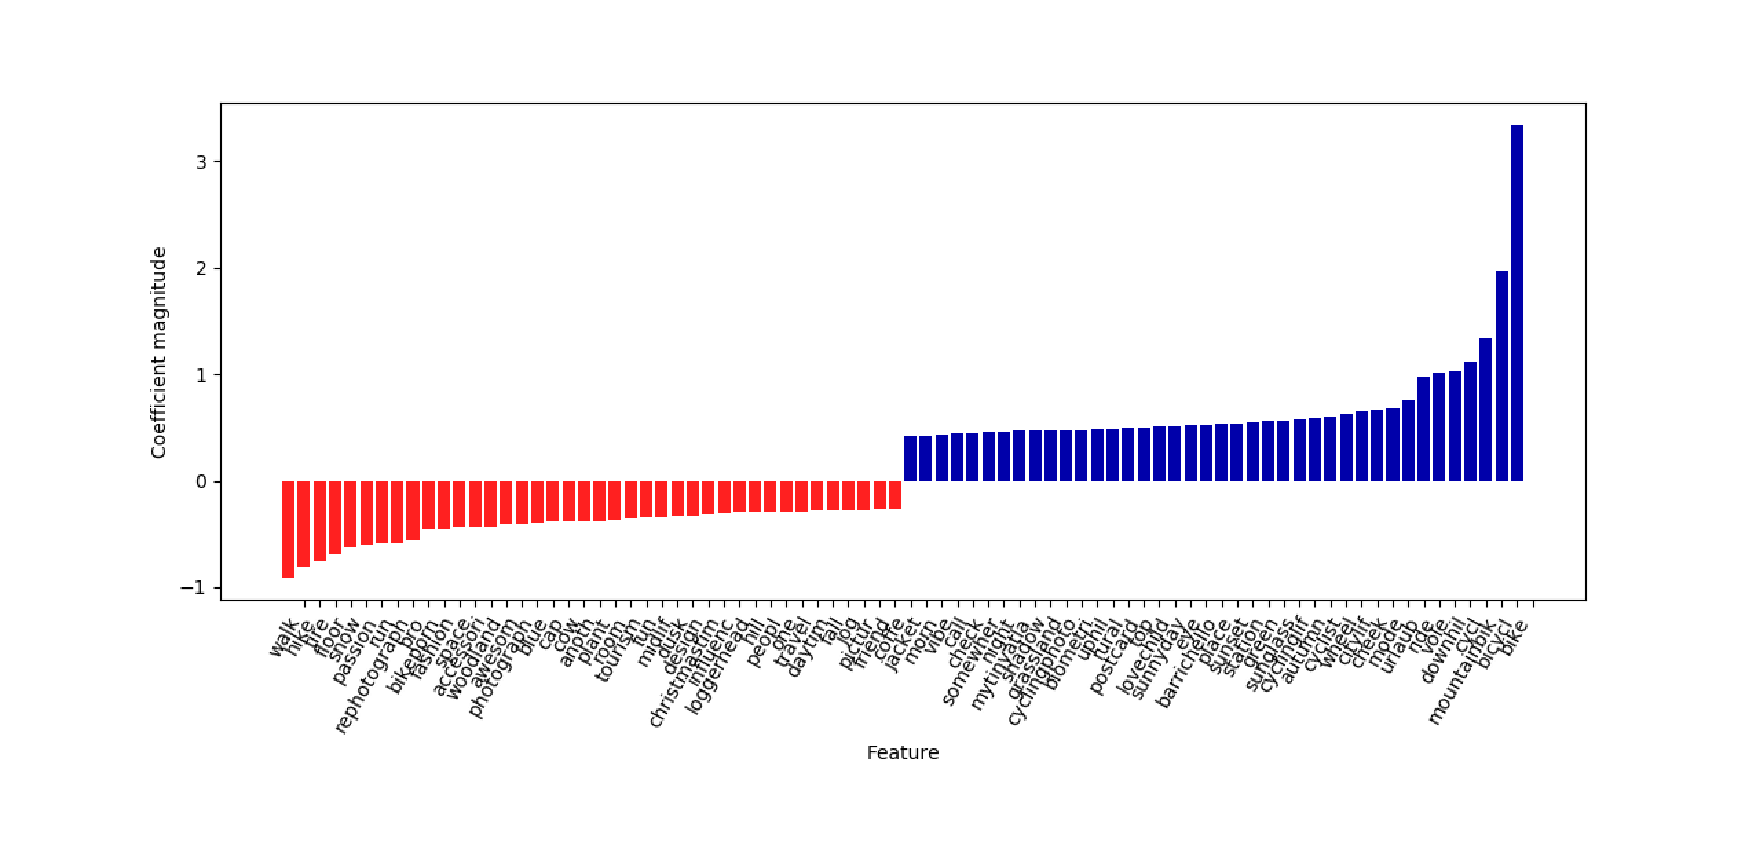
\includegraphics[width=\textwidth]{img/m2_top_40_features_Biking_cropped.pdf}
   \caption{Most predictive 40 M2-features of the class 'Biking'. Blue features are word-tokens which supports the presence of the corresponding classification. Red features support the opposite. The graphic was created with the \textit{mglearn} Python library provided by \parencite{Guido2016}}
   \label{fig:M2_top40_features_biking}
\end{figure}

\subsection{Model comparison}
In the following subsections, the above presented models will be thoroughly compared in terms of classification specific aspects, hyperparameter behaviour and performance on unseen data (data the models were not trained on). 

\subsubsection{Hyperparameter interaction}
The effect of different ngram\_range settings in combination with varying C values is illustrated in figure \ref{fig:heatmaps} for M1 and M2 respectively. The red circles indicates the highest F1-score present which corresponds to the best hyperparameter setting of the respective model (see table \ref{tab:m2_linearSVC_bestParams}). It becomes apparent, that the (2, 2) ngram\_range as well as the C value 0.01 underperform across the board. The F1-scores in the heatmaps are not completely identical to the values found in the corresponding model performance tables \ref{tab:m1_linearSVC_bestscores} and \ref{tab:m2_linearSVC_bestscores}. This variation is due to randomisation effects of the none-object selection from the database as well as from the model train and test splits (this is partly taken care of by cross-validation).\\

\begin{figure}[h!]
 \begin{subfigure}{0.5\textwidth}
   \centering
   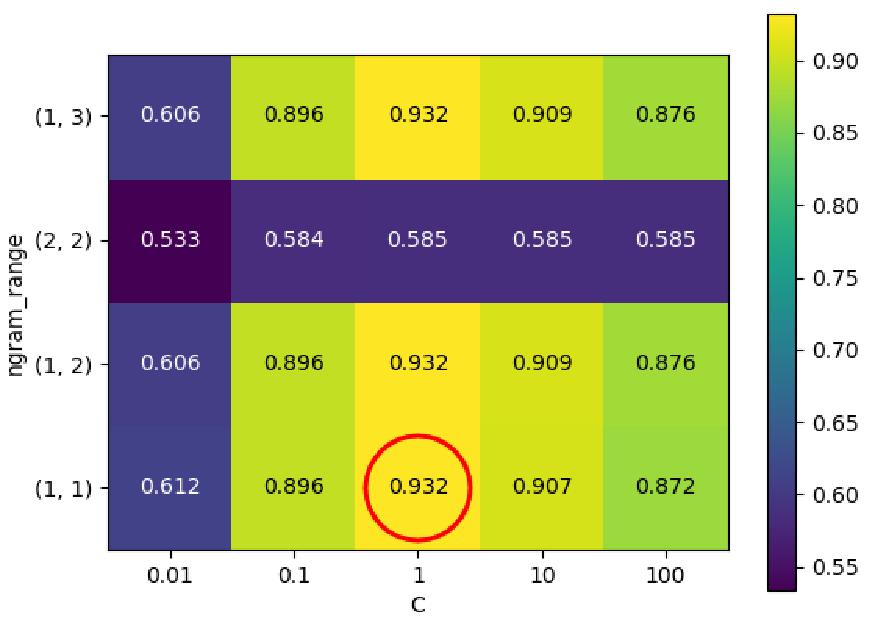
\includegraphics[width=0.9\linewidth]{img/m1_F1_ngram_C_heatmap_w_Circle.pdf}
   \caption{M1 linearSVC}
   \label{fig:m1_heatmap}
\end{subfigure}
\begin{subfigure}{0.5\textwidth}
   \centering
   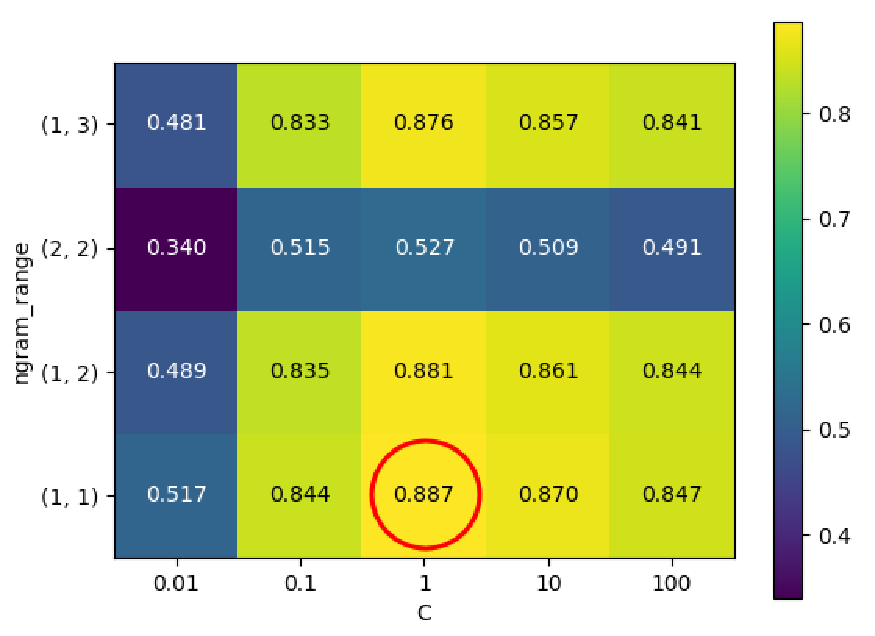
\includegraphics[width=0.9\linewidth]{img/m2_ngram_C_heatmap_new_w_circle.pdf}
   \caption{M2 linearSVC}
   \label{fig:m2_heatmap}
 \end{subfigure}
\caption{These heatmaps shows cross-validated F1-scores dependent on different combinations of the hyper-parameters ngram\_range and C for the model M1 (a) and M2 (b). These graphs were created with the Python library \textit{mglearn} from \parencite{Guido2016}}
\label{fig:heatmaps}
\end{figure}

\texttt{Remark:} If different hyperparameter settings produce the same model performance (F1-score) than the setting which produces fewer features is prioritised due to better generalisation capabilities. Regarding figure \ref{fig:m1_heatmap} for instance, the n\_gram setting of either (1, 1), (1, 2) or (1, 3) in combination with C = 1 all produce a F1-score of 0.932. (1, 1) has been chosen as best hyperparameter configuration due to the lowest feature count.

\subsubsection{Classification specific F1-scores}

\begin{figure}[h!]
   \centering
   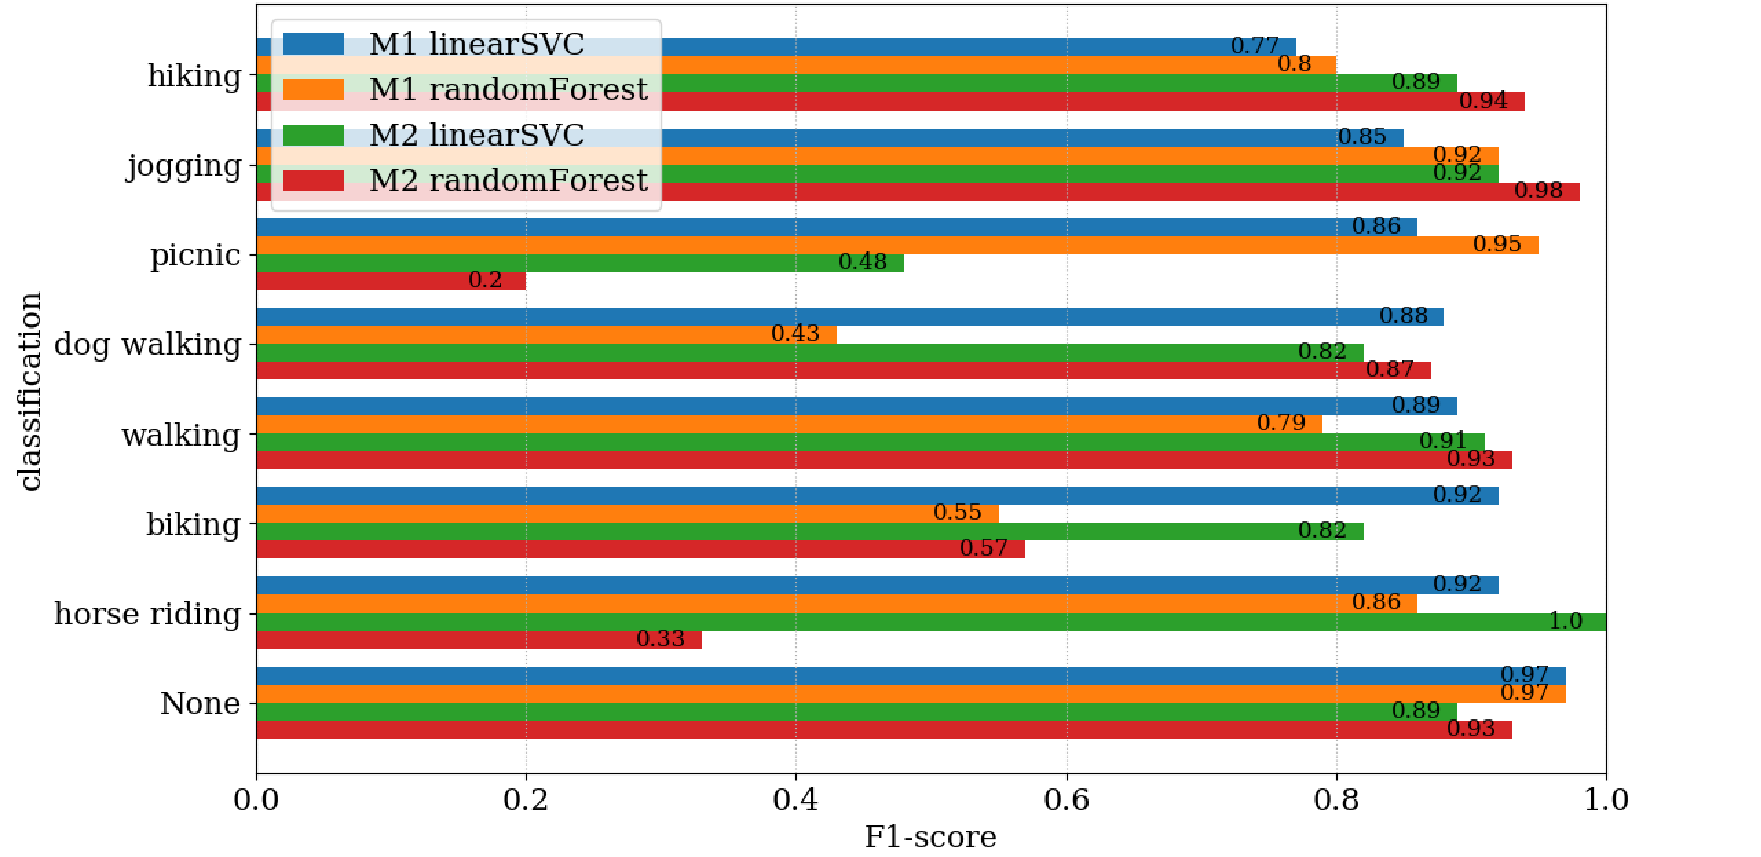
\includegraphics[width=\textwidth]{img/m1_m2_class_f1_scores_bigger_font.pdf}
   \caption{Comparison of the classification specific F1-scores of the linearSVC and random forest fitting algorithm of M1 and M2}
   \label{fig:m1_m2_class_f1_scores}
\end{figure}

\subsubsection{Final model scores}
In the end the model M1 and M2 were trained on the entire training's dataset which resulted in the following final performance scores visible in table \ref{tab:m1_m2_linearSVC_final_scores}. This step is important to generate a final model that is eventually trained on as much training's data as possible. Keeping a portion of the training's dataset aside for model validation is no longer necessary because the most well performing hyperparameter configuration was already determined before.\\
\newline
It can be noted at this point that the best M1 and M2 performance yielded similar feature counts during testing (626 and 775 respectively) and after training it on the entire dataset (845 and 958 respectively).  
\begin{table}[h]
\begin{center}
\caption{M2 linearSVC performance scores during testing (except accuracy train)}\vspace{1ex}
\label{tab:m1_m2_linearSVC_final_scores}
\begin{tabular}{cccccc}\hline
Model & Accuracy & Precision & Recall & F1 & F1 (without none class) & Features\\ \hline
M1 & 0.984 & 0.984 & 0.984 & 0.984 & 0.967 & 845\\
M2 & 0.991 & 0.991 & 0.991 & 0.991 & 0.993 & 958\\ \hline
\end{tabular}
\end{center}
\end{table}

\subsubsection{Precision on unseen data} \label{precision_unseen_data}
This section will present the results of the model performance on new data. All Instagram and Flickr media objects of the Canton of Zug on which these results are based were excluded from the M1 and M2 model training.\\
Two separate predictions per model were performed on the media objects contained in the following two database-tables (database overview see chapter \ref{database_setup}):\\
\texttt{media\_objects\_unionzug\_instagram} \\ \texttt{media\_objects\_cantonzug\_flickr}\\

One time the final text-string provided for the prediction was constructed by concatenating the processed text-data and the image labels of a given media object. The second time the final text-string only contained the processed text-data.\\

The model performance evaluation was done manually by the author. 100 media objects (if available) per class per prediction mode and per model were evaluated for True Positive (TP) or False Positive (FP) predictions. Only the model precision can be calculated with this information. An estimate for the recall over all classes was made based on the share of media objects that were correctly classified (except the none-class) in relation to the total amount of media objects present. In other words, how many media objects that actually contained NBRAs were also identified as such? This information is important because e.g. a model with 95\% precision that only identifies 20\% of media objects with a NBRA is still not practical. This approximation was calculated in the following way:

\begin{equation}
\label{equation_share_TP}
\frac{\sum_{class=1}^{7}(precision_{class}  * n^{total}_{class})}{n^{total}_{dataset}} * 100
\end{equation}
   
where the class-specific model precision (\textit{precision}\textsubscript{class}) is based on the evaluation of 100 media objects per class which can be a subset of the total amount of predicted media objects of that class.

\paragraph*{Model 1}
The best M1 accuracy of \textbf{0.764} was recorded for the media objects of the SMP Flickr while the parsed final text-string excluded image labels (see table \ref{tab:m1_actual_accuracy}). Predicting new data without image labels across both SMPs yields therefore an average model performance of \textbf{0.748}.\\
While the M1 accuracy differences between the two SMP's Instagram and Flickr was not significant on a 5\% level, the recorded differences between the inclusion and exclusion of image labels was significant.  
\begin{table}[h!]
\begin{center}
\caption{M1 NBRA prediction accuracy on unseen data}\vspace{1ex}
\label{tab:m1_actual_accuracy}
\begin{tabular}{ccc|c}\hline
SMP & +image labels & -image labels & \Delta\\ \hline
Instagram & 0.664 & 0.732 & -0.067\\
Flickr & 0.634 & 0.764 & -0.13\\
\hline
\Delta & 0.03 & -0.032 & \\ 
\end{tabular}
\end{center}
\end{table}

The incorporation of image labels into the final text-string results in a significant increase of overall and true positive predictions for both SMPs (see table \ref{tab:m1_actual_recall}).
In the case of Instagram the incorporation and exclusion of image labels results in a total of \textbf{668} and \textbf{384} NBRA-identifications which corresponds to 5.67\% and 3.26\% respectively of the 11'777 media objects in the database table \texttt{media\_objects\_unionzug\_instagram}.
In the case of Flickr the incorporation and exclusion of image labels results in a total of \textbf{273} and \textbf{67} NBRA-identifications which corresponds to 4.25\% and 1.77\% respectively of the 3'790 media objects in the database table \texttt{media\_objects\_cantonzug\_flickr}.\\
Therefore, the best performing final text-string format which excludes image labels results in a total of \textbf{451} (extrapolation based on the calculated precision on 100 media objects per class) true positive NBRA media objects across both SMPs. 

\begin{table}[h!]
\begin{center}
\caption{\%-share of correctly classified NBRA media objects through M1 (except the none-class) in relation to the entire dataset (according \ref{equation_share_TP})}\vspace{1ex}
\label{tab:m1_actual_recall}
\begin{tabular}{ccc|c}\hline
SMP & +image labels & -image labels & \Delta\\ \hline
Instagram & 5.67 & 3.26 & 1.74\\
Flickr & 4.25 & 1.77 & 2.4\\
\hline
\Delta & 1.424 & 1.493 & \\ 
\end{tabular}
\end{center}
\end{table}

\paragraph*{Model 2}
The best M2 accuracy of \textbf{0.776} was recorded for the media objects of the SMP Instagram while the parsed final text-string included image labels (see table \ref{tab:m2_actual_accuracy}). Predicting new data with image labels across both SMPs yields therefore an average model performance of \textbf{0.749}.\\
While the M2 accuracy differences between the two SMP's Instagram and Flickr was not significant on a 5\% level, the recorded differences between the inclusion and exclusion of image labels was significant.\\


\begin{table}[h!]
\begin{center}
\caption{M2 NBRA prediction accuracy on unseen data}\vspace{1ex}
\label{tab:m2_actual_accuracy}
\begin{tabular}{ccc|c}\hline
SMP & +image labels & -image labels & \Delta\\ \hline
Instagram & 0.776 &  0.691 & 0.085\\
Flickr & 0.721 & 0.753 & -0.032\\
\hline
\Delta & +0.055 & -0.062 & \\ 
\end{tabular}
\end{center}
\end{table}

The incorporation of image labels into the final text-string results in a significant increase of overall and true positive predictions for both SMPs (see table \ref{tab:m2_actual_recall}).
In the case of Instagram the incorporation and exclusion of image labels results in a total of \textbf{710} and \textbf{137} NBRA-identifications which corresponds to 6.029\% and 3.626\% respectively of the 11'777 media objects in the database table \texttt{media\_objects\_unionzug\_instagram}. In the case of Flickr the incorporation and exclusion of image labels results in a total of \textbf{227} and \textbf{82} NBRA-identifications which corresponds to 5.989\% and 2.164\% respectively of the 3'790 media objects in the database table \texttt{media\_objects\_cantonzug\_flickr}.\\
Therefore, the best performing final text-string format which includes image labels results in a total of \textbf{937} (extrapolation based on the calculated precision on 100 media objects per class) true positive NBRA media objects across both SMPs. 

\begin{table}[h!]
\begin{center}
\caption{\%-share of correctly classified NBRA media objects through M2 (except the none-class) in relation to the entire dataset (according \ref{equation_share_TP})}\vspace{1ex}
\label{tab:m2_actual_recall}
\begin{tabular}{ccc|c}\hline
SMP & +image labels & -image labels & \Delta\\ \hline
Instagram & 6.029 & 3.626 & 1.663\\
Flickr & 5.989 & 2.164 & 2.768\\
\hline
\Delta & 0.039 & 1.462 & \\ 
\end{tabular}
\end{center}
\end{table}

\paragraph*{Summary}
M1 and M2 showed in both cases the best performance if the parsed data for prediction (final text-string) was in the form the model was originally trained.\\
The model prediction accuracy was less dependant on the SMP the media objects originated from but more if image labels were parsed or not.\\
The best observed accuracy of M2 with \textbf{0.776} (average: 0.749) was only slightly better than the \textbf{0.764} of M1 (average: 0.748). Strong differences were registered in the percentage of correctly classified media objects in relation to the entire dataset which lay at roughly \textbf{6\%} for M2 but only at \textbf{1.8\%} for M1.
M2 with a slightly higher accuracy yielded (937-451=)486 more true positive NBRA-predictions than M1 which is an increase by factor two. Therefore M2 predicted less False Negatives (FN) which concludes that M2 also possess a \textbf{higher recall score} than M1 and generalises better on new data.



\section{Media object languages}
One assumption that was made earlier stated that the training's data from Zurich and the media objects from Zug share a similar written language by their author base. This would legitimise the usage of training's data that did not originate from the same region as the region the model would later be applied to.\\
To investigate on that assumption the five actively detected Instagram media object languages (see chapter \ref{langauge_detection}) of both regions (see figure \ref{fig:det_languages}) were compared with a paired two sample t-test for means. The result showed that the probability that T is smaller or equal t is 0.56 and therefore smaller than t\textsubscript{crit} of 2.78. Therefore, h0 (no difference present) cannot be rejected and the written languages of both areas are with high certainty of similar composition.

\begin{figure}[h!]
   \centering
   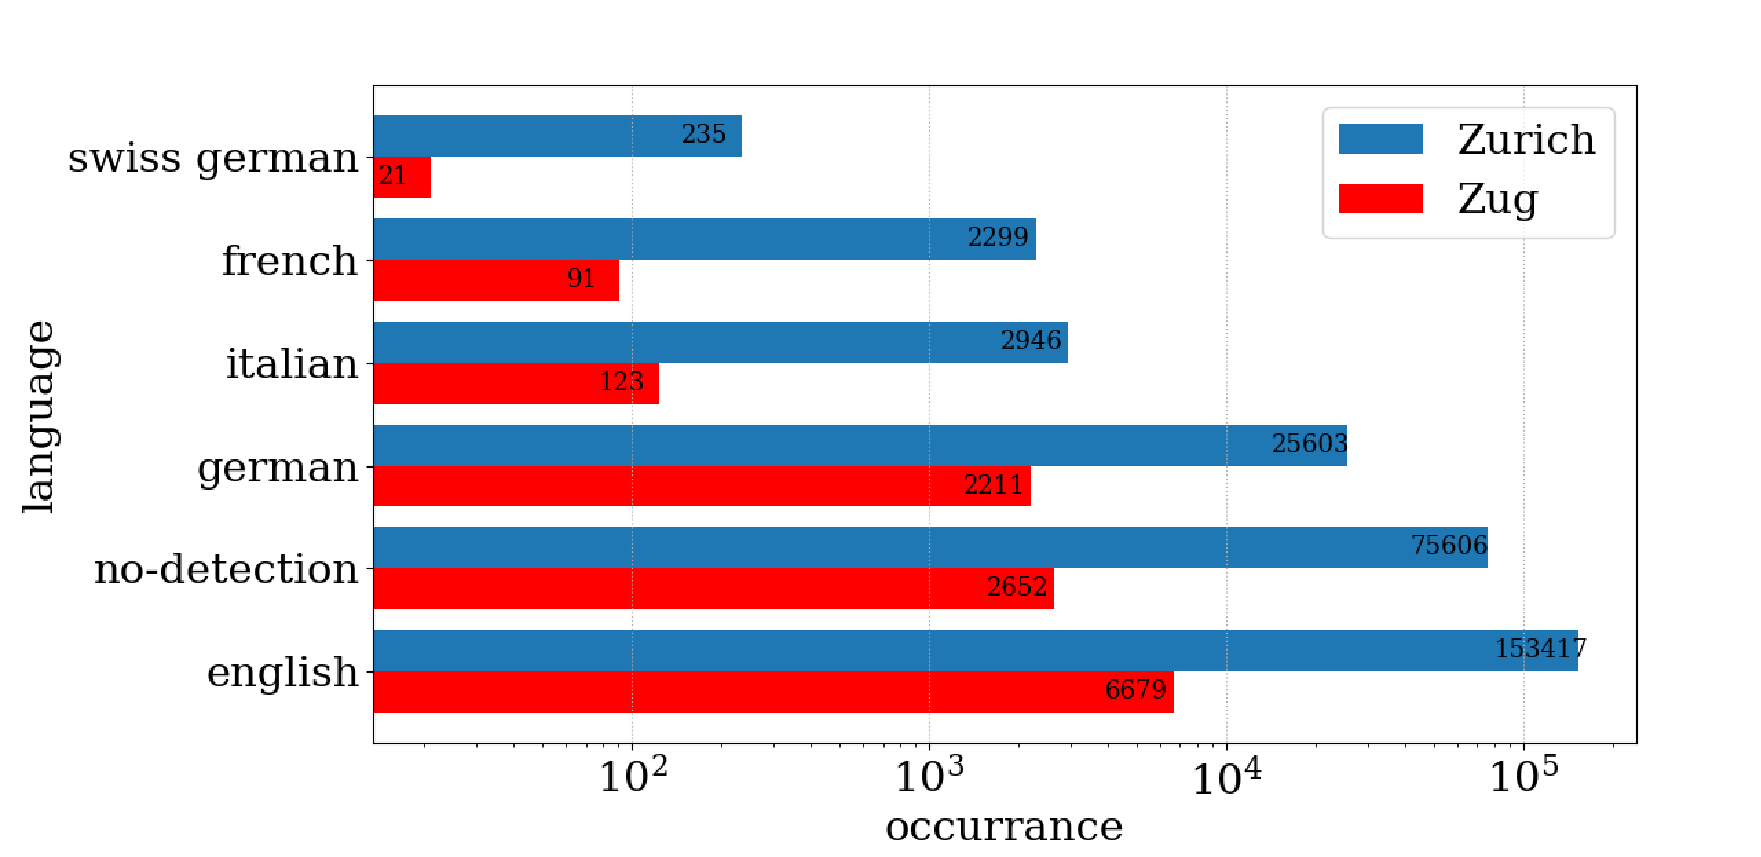
\includegraphics[width=\textwidth]{img/det_languages_bigger_font.pdf}
   \caption{Comparison between detected languages of Instagram media objects originating from Zug and Zurich}
   \label{fig:det_languages}
\end{figure}

\texttt{Remark:} Often times hashtags remain written in English due to their comprehensive meaning and purpose to connect media objects of similar content. Due to the big share hashtags normally have on the entire text, the language detection tends to identify a media object language as English above others.

\section{Ground truth evaluation}
The following subsections will cover the results from the \textit{in-situ} ground truth through passive observations and the 52 interviews over the three different locations 'Br\"uggli', 'R\"ossliwiese' and 'Schattenw\"aldli' (see chapter \ref{fig:locations_ground_truthing}) in the research area (Canton of Zug, Switzerland).

\texttt{Remark:} The entire data presented in the following subchapters is available on the enclosed CD to this thesis. This includes the actual transcript-data from the passive observation and the interviews (see chapter \ref{CD_content}).

\subsection{Passive observation analysis}
The passive NBRA-observation was performed by an assistant of the author. The thereby collected data is visible in figure \ref{fig:passive_observation} and shows the recorded NBRAs based on location sorted from left to right by decreasing observation frequency. Walking and hiking were by far the most recorded classes which corresponds to the interviews results visible in figure \ref{fig:interview_activities}. These two classes were merged due to differentiation difficulties just by observation and the demanded recording speed. 'Biking' follows second with a dominant occurrance in the location 'Br\"uggli' and no occurrence at 'R\"ossliwiese'. Third is 'jogging' shortly followed by 'dog walking' which have roughly the same occurrence frequency distribution across all three locations. 
\begin{figure}[h!]
   \centering
   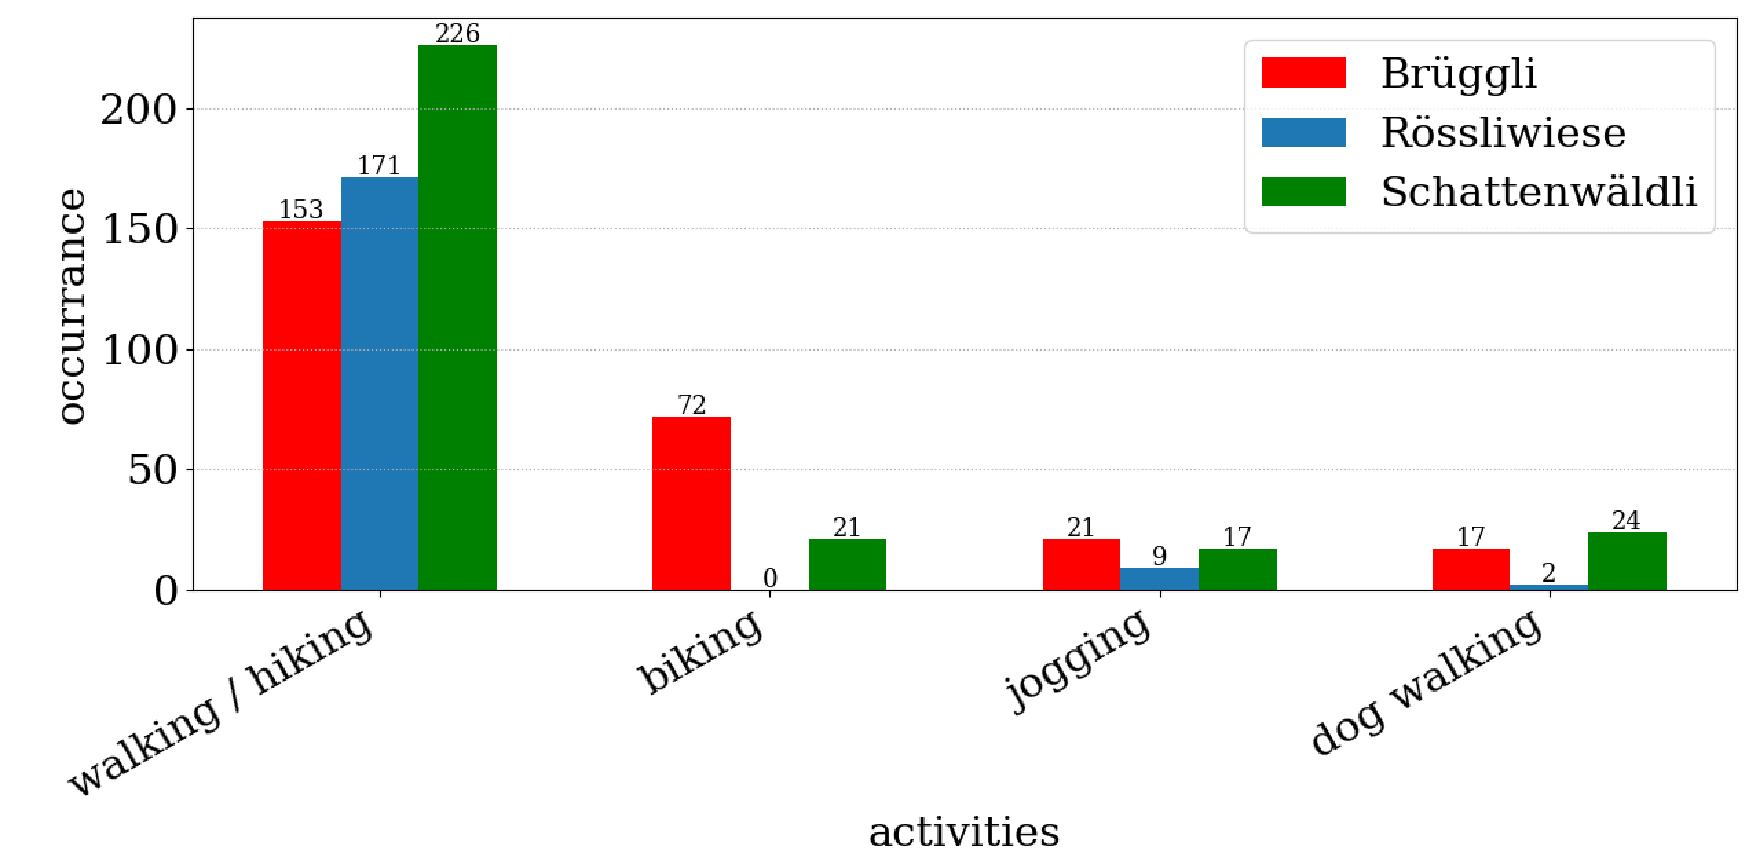
\includegraphics[width=\textwidth]{img/passive_observations.pdf}
   \caption{NBRA-occurrence according to the passive observation performed in the three locations listed in the legend}
   \label{fig:passive_observation}
\end{figure}

\subsection{Interview analysis}

\subsubsection{Occasion specific visitation motivations}
The top 8 motivations or reasons the interviewees mentioned why they visited a given location are displayed in figure \ref{fig:interview_visitation_motivation} sorted from left to right in descending order. According to the results plays 'Geographic closeness' a dominant role on how people decide upon their preferred recreation location. If a lake was present it was also frequently mentioned as a strong driver that draws in people for NBRAs. The argument 'sport' was solely mentioned for the location 'Schattenw\"aldli' and 'shopping', 'low traffic' and 'sunset' exclusively for the location 'R\"ossliwiese' and the term 'topography' for the location 'Br\"uggli'.

\begin{figure}[h!]
   \centering
   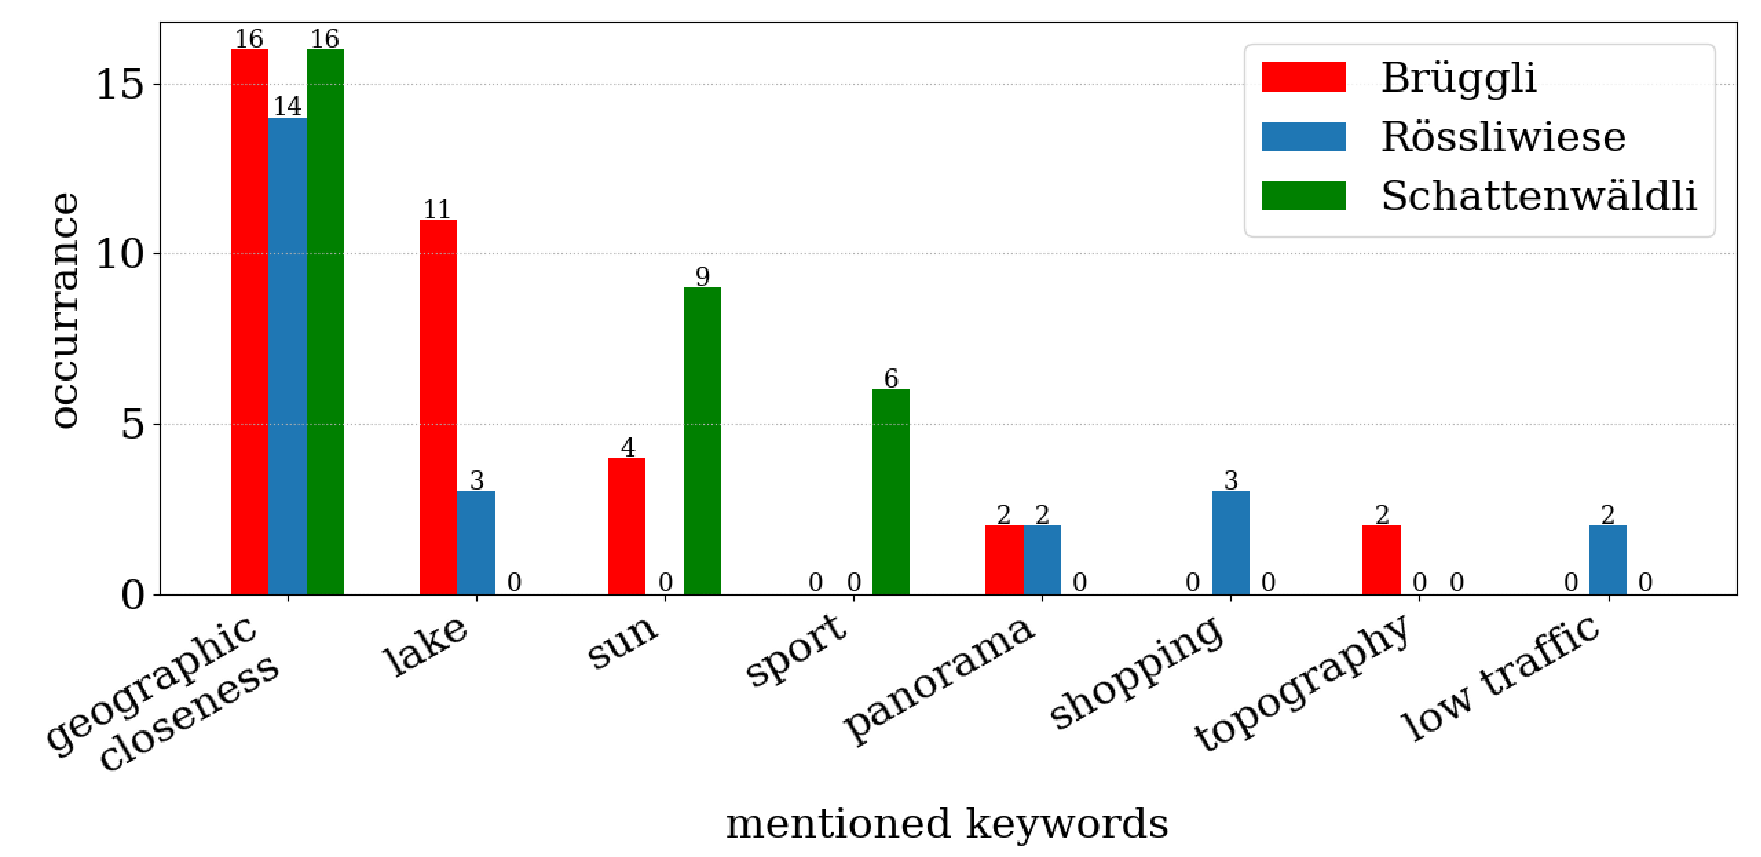
\includegraphics[width=\textwidth]{img/interview_keywords.pdf}
   \caption{Frequency of drivers mentioned by 52 interviewees for visiting one of the three locations listed in the legend.}
   \label{fig:interview_visitation_motivation}
\end{figure}

\subsubsection{Most frequent NBRAs performed by location}
Figure \ref{fig:interview_activities} is similar to figure \ref{fig:passive_observation} and shows similarly performed NBRAs. This time the descriptive term came from the interviewees themselves which explains why the differentiation between the classes 'walking' and 'hiking' was again established. 'Walking' still holds the biggest share across all three locations. 'Biking' follows again second and was recorded everywhere but in the location 'R\"ossliwiese' to which 'relaxing' was exclusive. Third comes 'hiking' which was only found on the mountain location 'Schattenw\"aldli'. The NBRA 'swimming' was not actively performed at the time of the interviews but it was instead mentioned by the interviewees as a regular summer activity at the location 'Br\"uggli'.
\begin{figure}[h!]
   \centering
   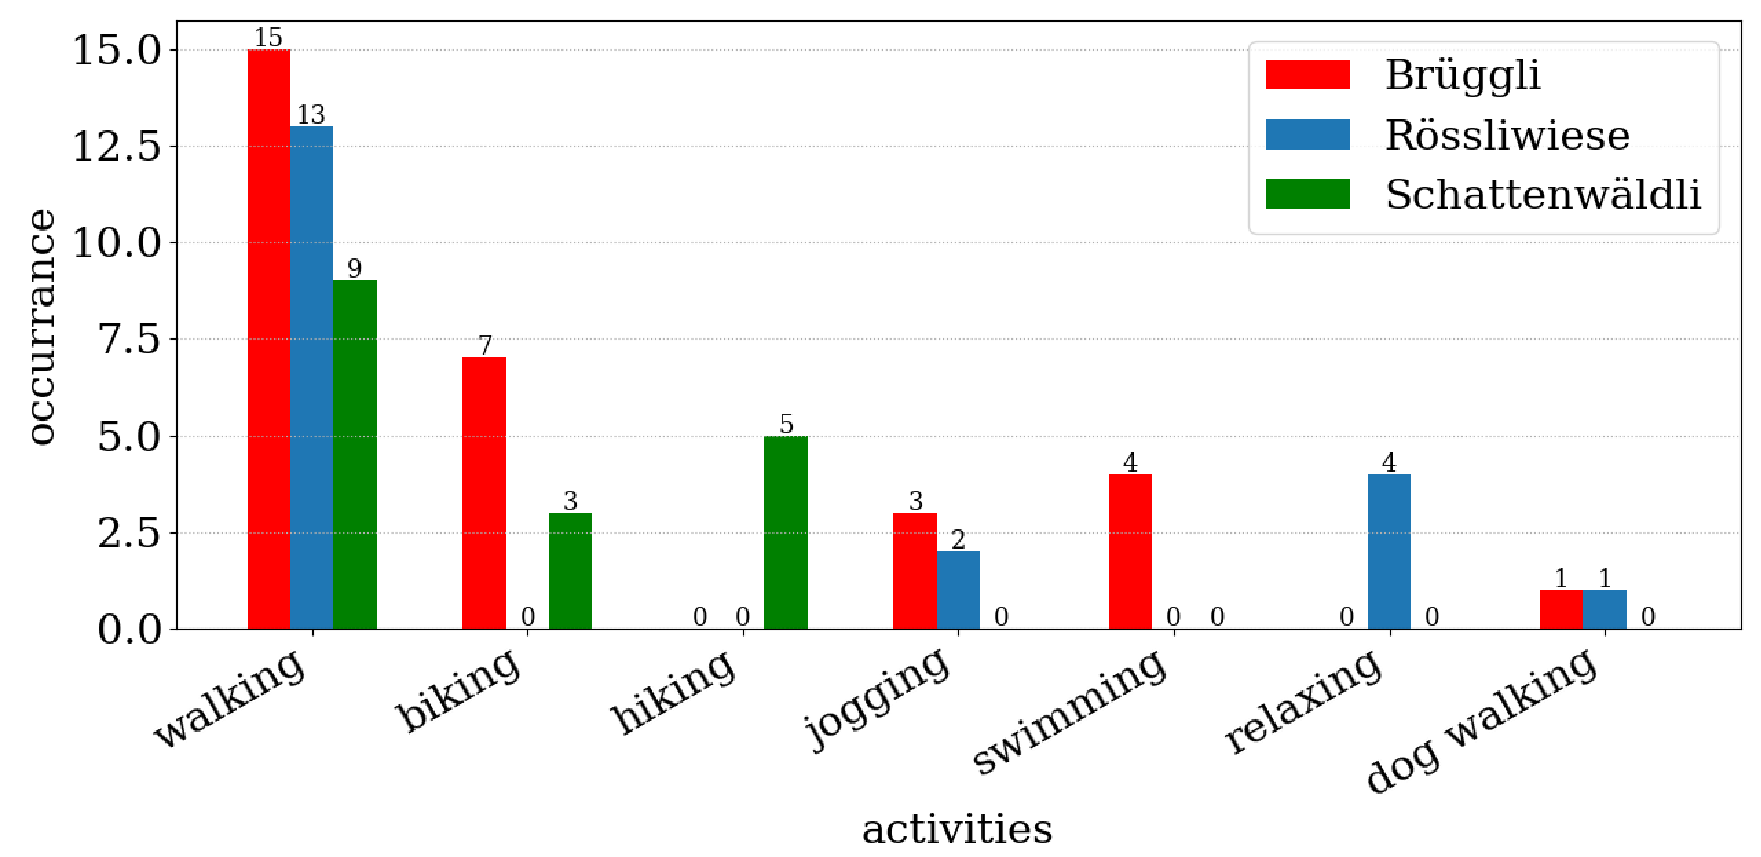
\includegraphics[width=\textwidth]{img/interview_activities.pdf}
   \caption{NBRA-occurrence according to the 52 performed interviews in the three locations listed in the legend}
   \label{fig:interview_activities}
\end{figure}

\subsubsection{Ranking of social media platform usage}
One main part of the interviews next to the information gain related to the performed NBRAs was dedicated to the interviewee's social media usage and engagement. Figure \ref{fig:interview_SMP} visualises the recorded occurrences where interviewees confirmed having an account on one of the given SMPs. Instagram and Facebook are by far the most widespread SMPs that were registered. LinkedIn follows third with less than half of the mentions of first or second place. Many interviewees mentioned the (sometimes forced) requirement of an LinkedIn account for their professional life.
A surprisingly low occurrence is registered for Twitter. STRAVA through being a specialised SMP was only mentioned once. Interestingly Flickr was not mentioned a single time during all 52 interviews.
\begin{figure}[h!]
   \centering
   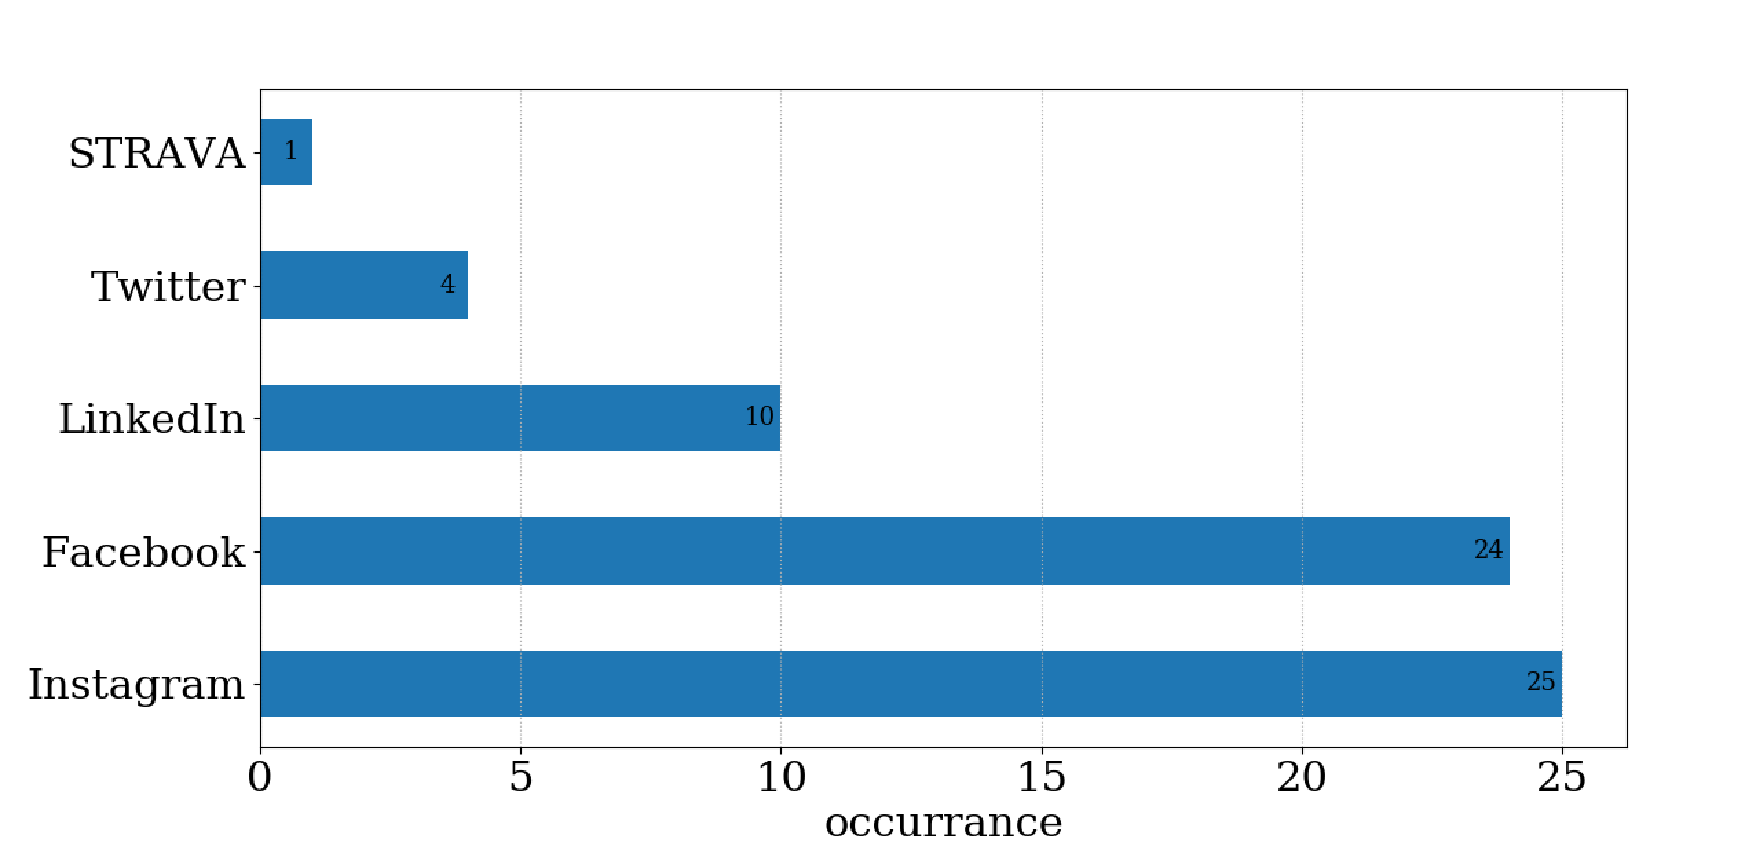
\includegraphics[width=\textwidth]{img/interview_socialmedia_bigger_font.pdf}
   \caption{Deviated SMP popularity according to confirmed profiles of 52 interviewees}
   \label{fig:interview_SMP}
\end{figure}

\subsubsection{Relation between age and social media presence}
Insight on dominantly represented ages groups in social media derived data can be drawn from figure \ref{fig:interview_age_SMP}. According to the 52 conducted interviews are people between the age of 21 and 30 most active on SMPs (red bars indicating a true participation). The age group of 61 to 100 on the other hand has not one recorded connection to any SMP. The red and blue line in figure \ref{fig:interview_age_SMP} represent the linear regression lines of the corresponding datasets. Their intersection can be found at roughly age 50 where the switch between the observed usage and absence of SMP's happens. Instagram and Facebook make out the biggest share of these records as already seen in figure \ref{fig:interview_SMP}. 
\begin{figure}[h!]
   \centering
   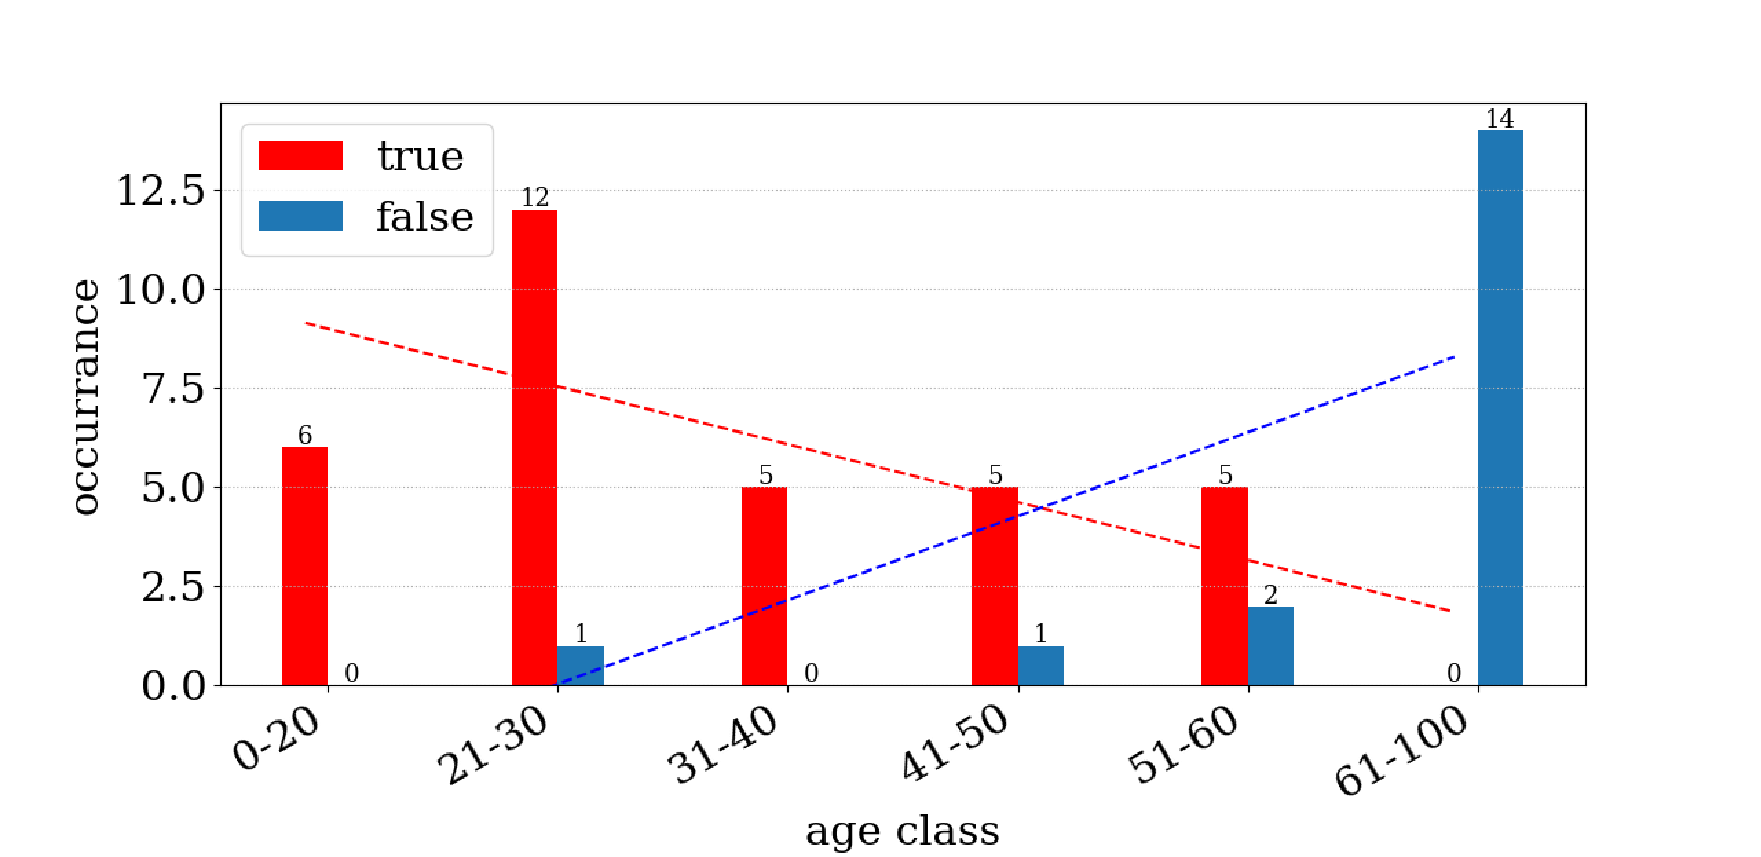
\includegraphics[width=\textwidth]{img/interview_socialmedia_age_bigger_font.pdf}
   \caption{Share per age class of social media users (true) and the once that do not use it (false). The red and blue line represent the linear regression of their corresponding datasets.}
   \label{fig:interview_age_SMP}
\end{figure}

\section{Spatial distribution of NBRAs}
This section will present the maps which resulted from the M2 NBRAs- prediction on both Instagram and Flickr media objects from the Canton of Zug. The cluster of maps in figure \ref{fig:map_cluster_2} show the NBRA's spatial distribution in parallel comparison between the two SMPs Instagram and Flickr. The amount of M2 predictions per classification and SMP are listed in figure \ref{tab:amount_class_NBRAs} as well as in the maps themselves as 'feature count'.

\begin{table}[h!]
\begin{center}
\caption{Amounts of M2 classified media objects that contain NBRAs}\vspace{1ex}
\label{tab:amount_class_NBRAs}
\begin{tabular}{cccc}\hline
Class & Instagram & Flickr & Total\\ \hline
Hiking & 231 & 126 & 357\\
Walking & 265 & 55 & 320\\
Dog walking & 143 & 16 & 159\\
Biking & 95 & 51 & 146\\
Jogging & 85 & 19 & 104\\
Horse riding & 37 & 6 & 43\\
Picnic & 23 & 6 & 29\\
 & & & \\
None & 10'898 & 3'511 & 14'409\\
\hline
\end{tabular}
\end{center}
\end{table}

As already described in chapter \ref{instagram_location_tag} Instagram locations can be user generated and are often general descriptions of the area at hand. This results in a lot of media objects being snapped to the same point on the map and therefore a lower spatial resolution. To illustrate this a bit further let's compare the two SMPs:
There are \textbf{152} unique Instagram locations of which the top three are named 'Zug' with 1'970, 'Canton of Zug' with 1'590 and 'lake Zug' with 400 associated Instagram media objects.
The processed Flickr dataset on the other hand consists of \textbf{1'144} unique locations of which the top three are named 'Baarerstrasse 12' with 112, 'Bahnhofsplatz' with 84 and 'Landsgemeindeplatz' with 69 associated media objects. This additional geo-information in form of an address is not provided by the \textit{Flickr API} by default but rather through the \textit{Google Geocoding API} as stated in chapter \ref{geocoding_api}.
One has to keep in mind that the processed Flickr dataset holds only roughly a third of the media objects compared to the processed Instagram dataset in the area of interest. 

\begin{figure}[h!]
   \centering
   \includegraphics[width=\textwidth,height=\textheight,keepaspectratio]{img/map_cluster_1.pdf}
   %\label{fig:map_cluster_1}
\end{figure}

\begin{figure}[h!]
   \centering
   \includegraphics[width=\textwidth,height=\textheight,keepaspectratio]{img/map_cluster_2.pdf}
   \caption{Spatial occurrence of NBRAs in the Canton of Zug based on M2 predictions which were conducted on text strings containing processed text-data and image labels from the Instagram / Flickr media objects.}
   \label{fig:map_cluster_2}
\end{figure}

\subsection{Comparison to ground truth}
Comparisons between the recorded NBRA-occurrences from the ground truthing consisting of the passive observation (see figure \ref{fig:passive_observation} and figure \ref{fig:interview_activities}) and the model were conducted to further evaluate its plausibility. 

\paragraph*{Biking}
The model predicts a strong occurrence of biking in the area of 'R\"ossliwiese' where the ground truthing consisting of the passive observation and the interviews did not record a single sighting (to the knowledge of the author: biking is not prohibited there and normally performed regularly).\\
In the area of 'Schattenw\"aldli' and 'B\"uggli' the ground truth recorded a moderate to strong occurrence of (mountain-)bikers. Only the former is also registered by the model. 

\paragraph*{Hiking}
'Schattenw\"aldli' is according to the interviews the only location of the three where interviewees said they performed the NBRA 'hiking'. The maps show also a strong signal of 'hiking' in the mountainous region. Inconsistency lies in the as 'hiking' classified media objects in the urban area of the city of Zug.

\paragraph*{Jogging}
The maps as well as the ground truth show moderate signals in all three locations and are therefore congruent.

\paragraph*{Walking}
M2 shows a predominant signal in the urban areas over the mountainous areas. Especially the lake side is strongly represented which coincides with the interviewee given motivation 'lake' listed in figure \ref{fig:interview_visitation_motivation} as well as with the performed activities in the locations 'Br\"uggli' and 'R\"ossliwiese' visible in figure \ref{fig:interview_activities}.

\paragraph*{Picnic}
The ground truthing did not yield any information on that classification.

\paragraph*{Dog walking}
The classification 'dog walking' is according to the ground truth performed in all three locations in a comparably low frequency similar to 'jogging'.  The M2 Instagram-data shows a signal densification in the urban area of the city of Zug whereas the Flickr-data shows a homogeneous distribution without any visible hot-spots.

\paragraph*{Horse riding}
The ground truthing did not yield any information on that classification.

\paragraph*{None} The M2 'None' classification signal shows as expected a homogeneous distribution (especially the Flickr-data with the higher spatial resolution) without any visible patterns. Because non-NBRAs were not actively recorded during the ground truthing, a direct comparison cannot be made.

\paragraph*{Summary}
Overall provides the model classification-specific spatial distribution patterns which were to be expected of the available ground truth data. Only 'hiking' shows some discrepancy and overlaps with the classification 'walking' which might be related to superordinate Instagram locations positioned in the urban areas. Refer to chapter \ref{XY} discussion for further insight/explanations on this topic. 


\subsection{Comparison to Foursquare}

\begin{figure}[h!]
   \centering
   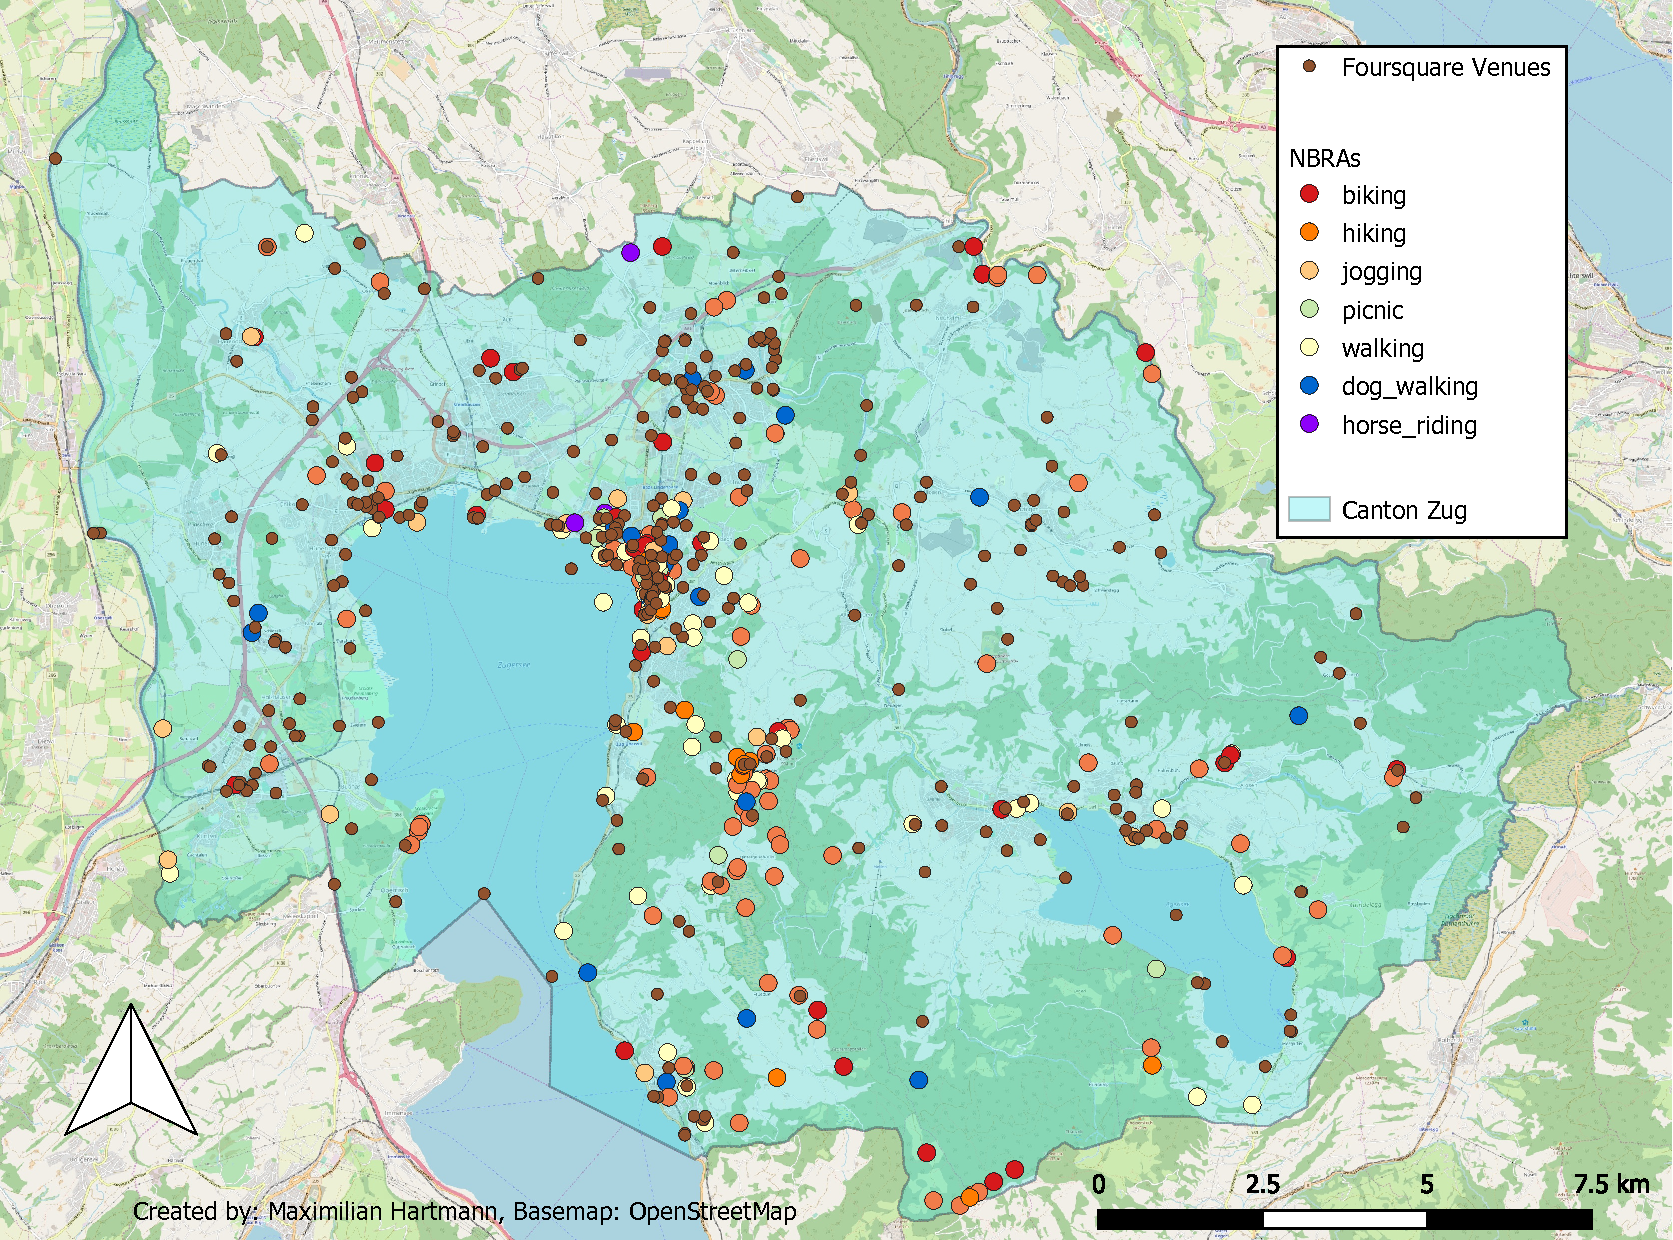
\includegraphics[width=\textwidth,height=\textheight,keepaspectratio]{img/foursquare_compare_cropped.pdf}
   \caption{Locations of all 404 Foursquare venues in relation to the M2 predicted spatial NBRA-occurrence.}
   \label{fig:map_foursquare_comparison}
\end{figure}


